% Espacio tangente: construcción vía curvas vs derivaciones
% Compilar con: pdflatex tangent_space.tex
\documentclass[tikz,border=10pt]{standalone}
\usepackage{tikz}
\usepackage{amsmath,amssymb}
\usetikzlibrary{arrows.meta, positioning, decorations.pathmorphing, calc}

\definecolor{gdlblue}{RGB}{41, 98, 168}
\definecolor{gdlred}{RGB}{191, 49, 49}
\definecolor{gdlgreen}{RGB}{30, 130, 76}
\definecolor{gdlorange}{RGB}{217, 130, 30}
\definecolor{gdlpurple}{RGB}{118, 56, 138}
\definecolor{gdlgray}{RGB}{140, 140, 140}
\definecolor{gdlyellow}{RGB}{190, 140, 10}

\begin{document}
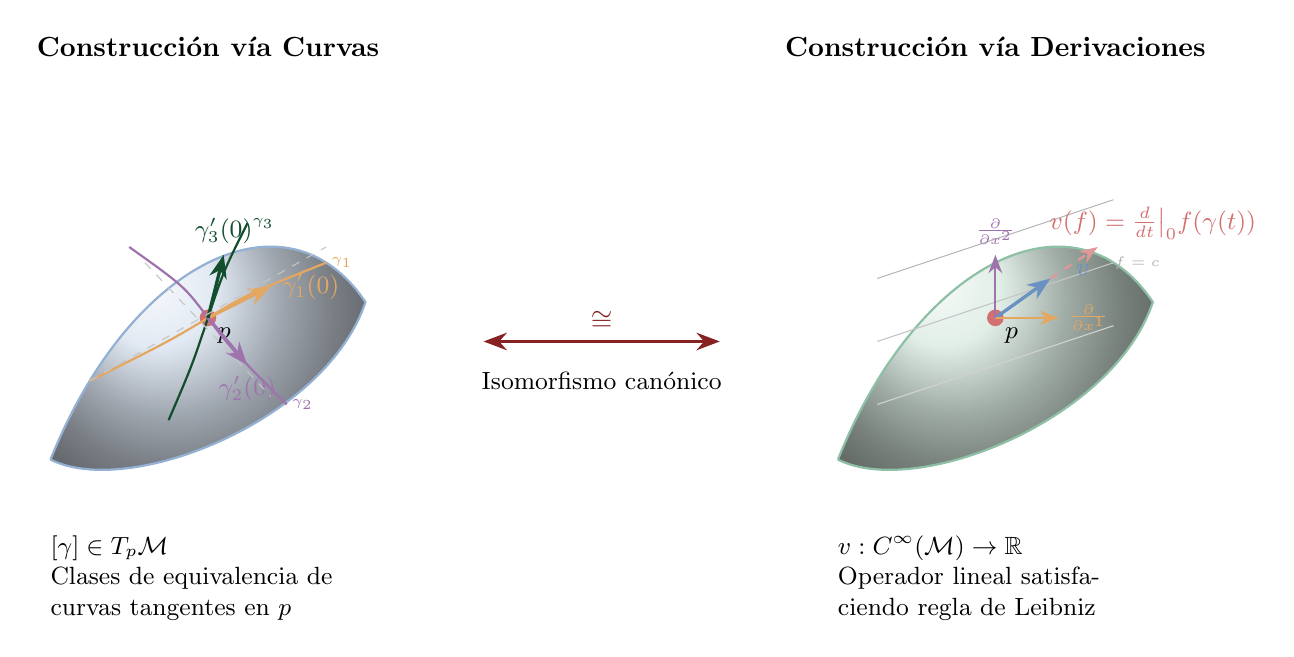
\begin{tikzpicture}[>=Stealth]

% === Panel izquierdo: Curvas ===
\begin{scope}[shift={(-5,0)}]
    \node[above, font=\bfseries] at (0, 3.5) {Construcción vía Curvas};

    % Superficie
    \shade[ball color=gdlblue!20, opacity=0.9]
        (-2,-1.5) .. controls (-1,1) and (1,2) .. (2,0.5)
        .. controls (1.5,-1) and (-1,-2) .. (-2,-1.5);
    \draw[thick, gdlblue!50]
        (-2,-1.5) .. controls (-1,1) and (1,2) .. (2,0.5)
        .. controls (1.5,-1) and (-1,-2) .. (-2,-1.5);

    % Punto p
    \coordinate (p) at (0, 0.3);
    \fill[gdlred!70] (p) circle (3pt);
    \node[below right, font=\small] at (p) {$p$};

    % Curvas pasando por p
    \draw[thick, gdlorange!70] (-1.5, -0.5) .. controls (-0.5, 0) .. (p) .. controls (0.5, 0.6) .. (1.5, 1);
    \node[gdlorange!70, font=\tiny] at (1.7, 1) {$\gamma_1$};

    \draw[thick, gdlpurple!70] (-1, 1.2) .. controls (-0.3, 0.7) .. (p) .. controls (0.3, -0.1) .. (1, -0.8);
    \node[gdlpurple!70, font=\tiny] at (1.2, -0.8) {$\gamma_2$};

    \draw[thick, gdlgreen!60!black] (-0.5, -1) .. controls (-0.2, -0.3) .. (p) .. controls (0.2, 0.9) .. (0.5, 1.5);
    \node[gdlgreen!60!black, font=\tiny] at (0.7, 1.5) {$\gamma_3$};

    % Vectores tangentes
    \draw[->, very thick, gdlorange!70] (p) -- ++(0.8, 0.4) node[right, font=\small] {$\gamma_1'(0)$};
    \draw[->, very thick, gdlpurple!70] (p) -- ++(0.5, -0.6) node[below, font=\small] {$\gamma_2'(0)$};
    \draw[->, very thick, gdlgreen!60!black] (p) -- ++(0.2, 0.8) node[above, font=\small] {$\gamma_3'(0)$};

    % Plano tangente (sugerido)
    \draw[dashed, gdlgray!50] (-1.5, -0.5) -- (1.5, 1.2);
    \draw[dashed, gdlgray!50] (-0.8, 1) -- (0.8, -0.7);

    % Etiqueta
    \node[font=\small, text width=4cm] at (0, -3) {
        $[\gamma] \in T_p\mathcal{M}$\\
        Clases de equivalencia de curvas tangentes en $p$
    };
\end{scope}

% === Panel derecho: Derivaciones ===
\begin{scope}[shift={(5,0)}]
    \node[above, font=\bfseries] at (0, 3.5) {Construcción vía Derivaciones};

    % Superficie
    \shade[ball color=gdlgreen!20, opacity=0.9]
        (-2,-1.5) .. controls (-1,1) and (1,2) .. (2,0.5)
        .. controls (1.5,-1) and (-1,-2) .. (-2,-1.5);
    \draw[thick, gdlgreen!50]
        (-2,-1.5) .. controls (-1,1) and (1,2) .. (2,0.5)
        .. controls (1.5,-1) and (-1,-2) .. (-2,-1.5);

    % Punto p
    \coordinate (p) at (0, 0.3);
    \fill[gdlred!70] (p) circle (3pt);
    \node[below right, font=\small] at (p) {$p$};

    % Función f representada como curvas de nivel
    \draw[gdlgray!40] (-1.5, -0.8) .. controls (0, -0.3) .. (1.5, 0.2);
    \draw[gdlgray!50] (-1.5, 0) .. controls (0, 0.5) .. (1.5, 1);
    \draw[gdlgray!60] (-1.5, 0.8) .. controls (0, 1.3) .. (1.5, 1.8);
    \node[gdlgray!70, font=\tiny] at (1.8, 1) {$f = c$};

    % Vector como operador diferencial
    \draw[->, very thick, gdlblue!70] (p) -- ++(0.7, 0.5);
    \node[gdlblue!70, font=\small, right] at (0.9, 0.9) {$v$};

    % Derivada direccional
    \draw[->, thick, gdlred!50, dashed] (0.7, 0.8) -- ++(0.6, 0.4);
    \node[gdlred!70, font=\small] at (2, 1.5) {$v(f) = \frac{d}{dt}\big|_0 f(\gamma(t))$};

    % Base
    \draw[->, thick, gdlorange!70] (p) -- ++(0.8, 0) node[right, font=\tiny] {$\frac{\partial}{\partial x^1}$};
    \draw[->, thick, gdlpurple!70] (p) -- ++(0, 0.8) node[above, font=\tiny] {$\frac{\partial}{\partial x^2}$};

    % Etiqueta
    \node[font=\small, text width=4cm] at (0, -3) {
        $v: C^\infty(\mathcal{M}) \to \mathbb{R}$\\
        Operador lineal satisfaciendo regla de Leibniz
    };
\end{scope}

% === Flecha de isomorfismo ===
\draw[<->, very thick, gdlred!70!black] (-1.5, 0) -- node[above, font=\normalsize] {$\cong$} (1.5, 0);
\node[font=\small] at (0, -0.5) {Isomorfismo canónico};

\end{tikzpicture}
\end{document}
